\documentclass[10pt,conference,letterpaper]{IEEEtran}
\usepackage{graphicx}
\usepackage{soul}
\usepackage{balance}

% pete's adds
\usepackage{color}
\newcommand{\todo}[1]{{\textcolor{red}{#1}}}
\newcommand{\blue}[1]{{\textcolor{blue}{#1}}}
\newcommand{\pjk}[1]{[\todo{PJK: #1}]}
\newcommand{\bjb}[1]{[\blue{BJB: #1}]}

\newcommand{\pjkst}[2]{[\todo{PJK: #1}]\st{#2}}
\newcommand{\note}[1]{\textcolor{blue}{[#1]}}
\newcommand{\red}[1]{\textcolor{red}{#1}}
\newcommand{\dspace}{\renewcommand{\baselinestretch}{1.04805}\Large\normalsize}

\begin{document}
\dspace

\title{Geo-Replicating Federated File Systems}
\author{\IEEEauthorblockN{Benjamin Bengfort and Pete Keleher}
\IEEEauthorblockA{Department of Computer Science\\
University of Maryland, College Park, MD, USA\\
\{bengfort,keleher\}@cs.umd.edu}}

% - novel wide area distributed FS
% - introduce user-centric dynamic networks
% - implementation of a geographically distributed FS with Raft and anti-entropy
% - flexible consistency model (could expand this)
% - file system consistency model (forks etc)
% - forte number
% - evidence that a centralized quorum provides benefits a la Oceanstore/Gray
%
% Maybe we can sell this as a simple idea that may have off-handedly been mentioned but
% that we've explored in detail and discovered that there are  tricky bits that have to be
% resolved?

\date{December 12, 2016}

\IEEEtitleabstractindextext{%
\begin{abstract}
Groups of strongly consistent devices can efficiently order events under
ideal (data center) conditions, but become less effective in dynamic and
heterogeneous environments.  Eventually consistent devices efficiently
tolerate both faults and dynamic conditions but are slow to converge on a
single ordering of system events.

We propose ``federated consistency'', which combines the strengths
of both approaches into a single protocol, and show how to map a distributed
file system onto a federated system.  Federated groups use a strongly
consistent inner core of devices to maintain a totally ordered, fault-tolerant
sequence of events.  A cloud of eventually-consistent devices disseminates
orderings and enables progress despite varying connectivity and partitions.
Though the constituent sub-protocols take different (nearly opposite)
approaches to resolving conflicts; we show that use of a forte number allows
them to inter-operate effectively.  We use a discrete event simulation to show
that a group of federated devices can obtain the key advantages of both
approaches.
\end{abstract}}

\maketitle

\IEEEdisplaynotcompsoctitleabstractindextext

\section{Introduction}


The rise of on-demand computing resources and the Cloud has made distributed systems the
default approach to scaling applications for many users in a variety of geographic
locations.
In particular, data replication is used to increase availability, throughput, durability,
and fault tolerance by ensuring that objects can be accessed on multiple servers as
locally as possible.
Although some coordination is necessary to ensure that replication happens correctly, many
systems favor a relaxation in consistency in order to meet the performance requirements of
modern, mobile applications.
This is partially because the application layer can define its own mechanisms for handling
differently consistent behavior but it is primarily because such systems are implemented
in data center contexts that enjoy stable, low-latency connections which allow optimistic
approaches and provide consistent views of data \emph{most of the time}
\cite{bailis_quantifying_2014,bermbach_metastorage:_2011}.

We might, therefore, generally categorize most modern distributed storage systems and
NoSQL databases as not having strong consistency and using some consensus algorithm for
control and synchronization when necessary.
As a result consistency is usually described in a discrete, data-centric fashion: weak or
strong; eventual, causal, or sequential and no longer described in client-centric terms
\cite{bermbach_consistency_2013}.
As replication becomes more prevalent, however, it is not enough to simply lay the burden
of conflict at the feet of clients and there has been recent interest in instead
redefining consistency along a spectrum whose dimensions are the strictness of ordering
writes and the potential staleness of reads
\cite{yu_design_2002,li_making_2012,afek_quasi-linearizability:_2010,al-ekram_multi-consistency_2010,krishnamurthy_adaptive_2002}.

By defining consistency in terms of ordering and staleness it is easy to see that the root
cause of the tradeoff between performance and correctness is message latency, where a
common case is when messages do not or cannot arrive due to node failure or network
partitions.
It has been noted that message latency is the key factor in determining ``how consistent''
a system is either due to staleness in eventually consistent systems
\cite{bailis_probabilistically_2012} or by preventing progress in sequential consistency
systems implemented with consensus \cite{howard_raft_2015}.
The advent of distributed storage as a service has allowed systems to adapt consistency at
runtime by taking advantage of a stable network environment
\cite{chihoub_harmony:_2012,chihoub_consistency_2013,kraska_consistency_2009,pitoura_data_1999,deno-toc} and has
shifted the focus away from replication in weakly-connected, dynamic, or mobile networks.
We believe that local, user-oriented distributed systems should augment
cloud services rather than be replaced by them; and in some cases, such as disaster
recovery or search and rescue, may be the only available system.

In this paper we present a novel approach to flexible consistency via the federation of a
heterogeneous system of replica servers that implement a variety of consistency protocols
in response to local policies and requirements.
As a result, individual replicas in the system can respond and adapt to a changing network
environment while providing as strong a local guarantee or minimum quality of service as
required.
The global state of a federated system is defined by the replica topology and their
interactions, such that if a subset of replicas implement stronger consistency models,
then the global probability of conflict is reduced.
Conversely, a subset of replicas implementing a weaker consistency can increase global
throughput.
Indeed, we find that it is more often the tension between local vs global views of
consistency that cause greatest concern in terms of application performance.
Because each node can select and change local consistency policies, client applications
local to the replica server have greater control of tuning consistency in response to
mobile or dynamic network behavior, maximizing timeliness or correctness as needed.

We show that a federated consistency protocol can find a middle ground in the trade-off
between performance and consistency, particularly between an eventually consistent system
implemented via gossip-based anti-entropy \cite{kempe_gossip-based_2003} and a sequential
consistency model implemented by the Raft consensus protocol \cite{ongaro_search_2014}.
By exploring these two extremes in the consistency spectrum we show that the overall
number of inconsistencies in the system is reduced from the homogeneous eventual system and
that the access latency is decreased from the homogeneous sequential system.
Moreover, because the global consistency of the system is topology-dependent, it can be
said to have flexible or dynamic consistency.
We have found that large systems with variable latency in different geographic regions can
perform well by allowing most nodes to operate in an optimistic fashion, but also maintaining a
strong central quorum to reduce the amount of global conflict.

The rest of the paper is organized as follows: Section~\ref{sec:background}
describes background and defines terms. Section~\ref{sec:replication}
describes implementations of eventually consistent and Raft clouds, focusing on
the non-standard aspects of our approach, which are intended to support
file systems in wide-area and mobile environments.
Section~\ref{sec:federated} describes our Federated protocol with eventual and
sequentially consistent sub-protocols.
Section~\ref{sec:results} explores simulated performance of the three
protocols, Section~\ref{sec:related} describes related work, and Section~\ref{sec:conclusion} concludes.

\section{Background and Definitions}
\label{sec:background}

Our target environment is wide-area: we assume
replicas are distributed across
multiple geographic regions, where communication within a region is fast and
cheap but inter-region communication is expensive.
We define consistency in terms of the ordering of operations that change the
state of a replica.
In the context of a wide-area file system, those operations could be individual
\texttt{write()} systems calls, though this would be inefficient.
Most wide-area file systems aggregate individual accesses through
\textit{Close-To-Open} (CTO) consistency, where file reads and writes are
``whole file'' \cite{afs,coda,lbfs}.
A file read (``open'') is guaranteed to see data written by the latest write
(``close'').
This approach satisfies two of the major tenets of session consistency:
\texttt{read-your-writes} and
\texttt{monotonic-writes}, but not
\texttt{writes-follow-reads}~\cite{bermbach_consistency_2013,terry_session_1994,vogels_eventually_2009}.

The system operations to be replicated are therefore a series of file writes.
Each file has meta-information that includes a unique name and a monotonically
increasing version number.
%  which can be implemented either as a vector clock
% \cite{parker_detection_1983} (or a simple Lamport scaler) in the case of a fixed topology
% or as a vector timestamp \cite{almeida_version_2002} in the case of dynamic
% topologies.~\pjk{I don't think this is true.}
A file write includes the file name, the parent version of the file to which the write is being applied,
versions and names of any other dependencies, the replica ID where the write
occurred, and an array of blob IDs that determine the file data at
the conclusion of the write.
A file read simply looks up the latest local version of that file.
% Because dependency information can be embedded into a write, it is not necessary to
% include read accesses in the log.

% For example, in order to create a transaction that reads from objects $X$ and $Y$,
% performs a computation then updates objects $Y$ and then $Z$: the write to $Y$ would
% include as a dependency the earlier version of $Y$ and the read version of $X$ and the
% write to $Z$ would include the updated version of $Y$ and the read version of $X$.
% Other notions of dependencies include implicit session dependencies, e.g.
% all writes are dependent on any access that occur within a minimum time threshold of each
% other, or explicit dependencies that are added by the application.
% \pjk{why are we talking about transactions and embedded depencies?}

Our file system, like many modern file systems,
decouples
meta-data~\emph{recipes}~\cite{tolia:opportunistic,gfs,shvachko2010hadoop,ross2000pvfs,globalfs}
from file
data storage.
Meta-data includes an ordered list of \emph{blobs}, which are opaque binary chunks.
When a file is closed after editing, the data associated with the file is \emph{chunked} into a
series of variable-length blobs~\cite{lbfs}, identified by a hashing function applied to
the data~\cite{rabin}.
Since blobs are effectively immutable~\cite{helland_immutability_2015}, or tamper-evident, (blobs are named by hashes of
their contents), we assert that consistent meta-data replication can be decoupled from blob
replication.
Accesses to file system meta-data becomes the operations or entries in replicated logs.
Meta-data is therefore replicated through the system, allowing any file
system client to have a complete view of the file system namespace, even while
not caching any file data.

\subsection{Operation Logs}

Meta-data writes are replicated and appended to per-replica \emph{logs}.
Consistency is therefore expressed in terms of the ordering of an operation log,
replicated across all system replicas, where operations consist solely of file
writes.
If all logs are identical, the same file writes are applied in the same order
at each replica, and the file system will appear the same on all replicas.
As such,
we use a {data-centric} model of correctness that concentrates primarily on
two metrics: log operation ordering and read
staleness~\cite{bermbach_consistency_2013}:
\begin{enumerate}
\item \emph{Ordering} refers to how closely individual logs adhere to the abstract
  global ordering. A strict ordering requires every single log to be exactly the
  same, whereas weaker ordering allows some divergence in the order writes are stored in
  the log.
\item \emph{Staleness} refers to how far local logs are behind the latest version of the log globally,
  and can be either expressed by the average latency of replicating new versions, or
  simply by how far behind the average replica is from the latest log.
\end{enumerate}

Most data-centric consistency models do not consider staleness, but instead refer to
guarantees on ordering strictness and the method by which updates are applied to the state
of the replica.
However, the goals of strict ordering and minimal staleness can be in conflict. For
example, a strict ordering criteria may require a new object version to be delayed until
dependencies are satisfied, causing reads to become more stale.

\subsection{Forks}

In addition to tracking staleness directly, we also use as a metric the primary symptom of stale
reads and writes, forks:
\begin{quote}
    A \emph{fork} occurs when two replicas concurrently write a new version to the same parent object.
\end{quote}
Forks introduce inconsistency because they allow multiple potential orderings of operation
logs.
Forks are primarily a symptom of staleness; e.g. the second writer wrote to
a stale version of the object.

\begin{figure}[t]
    \centering
    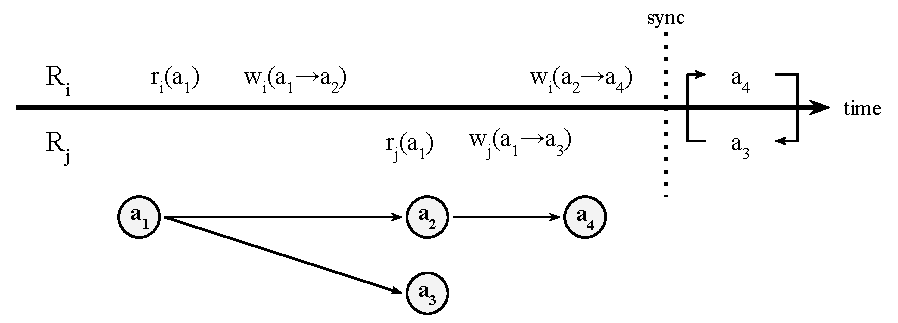
\includegraphics[width=0.5\textwidth]{figures/forks}
    \caption{Accesses before synchronization cause stale reads and forked writes.}
    \label{fig:forks}
\end{figure}

Almost all consistency models, with the exception of
\textit{linearizability}~\cite{herlihy_linearizability:_1990}, are susceptible to forks
because they allow stale reads to occur.
Object \emph{coherence} requires an object's version history to be a linear sequence.
Object forks violate coherence and occur, for example, when replicas $i$ and $j$ read object version $a_1$
and then concurrently attempt to write new versions: $W_i(a_1 \rightarrow a_2)$ and
$W_j(a_1 \rightarrow a_3)$ (Figure~\ref{fig:forks}).
A delay in replicas $R_i$ and $R_j$ synchronizing could lead to one of them continuing
further down one of the fork paths, e.g. $W_i(a_2 \rightarrow a_4)$.
Forks can be caused by concurrent reads, but the fork between $a_2$ and $a_3$
actually occurs because $R_j$'s read is stale.

Note that if the \texttt{sync} line were moved back \emph{before} $R_j$'s read,
the read would no longer be stale and $a_2/a_3$ would not constitute a
fork. However,  $a_3/a_4$ would then be a fork.

\subsection{Consistency}

A broader discussion of consistency levels should include at least eventual consistency~\cite{terry_managing_1995},
causal consistency~\cite{causal} (the highest level allowing high availability~\cite{bailis_bolt-causal_2013}),
sequential consistency~\cite{sequential-consistency}, and linearizability~\cite{herlihy_linearizability:_1990}.
For reasons of space, however, we limit this discussion to the models most
useful for our purposes:
eventual and sequential consistency.

\emph{Eventually consistent} logs, no matter their ordering, must eventually have identical final
writes for each object in the namespace (recall that writes are whole-file with CTO consistency).
This suggests that eventual consistency requires some \textit{anti-entropy} mechanism to
propagate writes and a policy to handle convergence \cite{terry_managing_1995}.
Eventual consistency is very popular for NoSQL databases and hosted distributed storage
services \cite{decandia_dynamo:_2007,lakshman_cassandra:_2010} because it allows
optimistic implementations.
Conflict resolution is often left to the application layer, but
in practice most applications can handle some inconsistency.
The low latencies in cloud data centers often make windows of
inconsistency rare and
short-lived enough to be tolerable~\cite{bailis_quantifying_2014}.

Eventual consistency convergence implemented by a \textit{last writer wins} policy simply accepts all
writes so long as they are more recent than the latest local versions.
Reads and writes are always performed locally, and therefore with little
performance overhead.
Eventually consistent logs may temporarily diverge as long as the final versions of each
object eventually converge.
As a result, the current version of an object on a single replica may alternate between writes to competing
forks (a fairly weak semantic); it is up to the application to detect and compensate for the
inconsistency.

\emph{Sequentially consistent} logs must be ordered identically, though the logs of
lagging replicas may only be prefixes of the latest log in the system~\cite{attiya_sequential_1994}.
Sequential consistency does not make guarantees about staleness
(or the ordering of reads) but does require that all writes become visible in the same
order \cite{bermbach_consistency_2013}.
Sequentially consistency can be implemented with consensus algorithms such as Paxos
\cite{lamport_fast_2006} or Raft \cite{ongaro_search_2014} that coordinate logs by
defining a transitive, global ordering for all conflicts.
Alternatively, sequential consistency can be implemented with warranties -- time-based
assertions about groups of objects that must be met on all replicas before the assertions
expire~\cite{liu_warranties_2014}.

Stale reads are possible because of lagging replicas.
However, only a single branch of a forked write can be committed to any copy of the log.
Preventing forks would require either a locking mechanism or an optimistic approach that
allowed operations to occur but rejects all but one branch (the approach discussed in our
Raft implementation below).
Write rejection requires the application to deal with dropped writes by either retrying or
resolving conflicts and writing a new version.

\section{Replication}
\label{sec:replication}
A federated consistency model allows individual replicas to
engage in replication according to locally-specified consistency policies.
Each replica maintains its own local state, modified in response to local accesses
and receipt of messages from remote replicas.
Each replica sends messages to other replicas in order to propagate new writes.
Therefore every replica can be seen as an event handler that responds to local access
events, as well as remote messages, and generates more events (sent messages) in return.
So long as every federated replica has an event handler for all types of RPC
messages, federation primarily has to be defined at the \textit{consistency boundaries},
that is when replicas of one consistency type send messages to that of another.

% Given the consistency models discussed in the previous section, we will omit weak
% consistency as being too simplistic and linearizability as being too performance
% restrictive.
% Instead we will focus on the federation of eventual consistency, implemented with
% latest-writer wins gossip based anti-entropy, and sequential consistency implemented with
% the Raft consensus algorithm.

\subsection{Gossip-Based Anti-Entropy}

Eventually consistent replicas  read and write locally without remote communication delays.
Writes are propagated among replicas through
periodic \textit{anti-entropy} sessions that
converge replicas towards the same state (e.g.
reducing entropy, the divergence between the states of individual replicas)
\cite{kempe_gossip-based_2003}.
At routine intervals specified by the \texttt{anti-entropy delay} timing parameter, a
replica will randomly select one of the other replicas in the system and send a
\texttt{Gossip} message that logically contains the latest version of all objects in the replica's
local log.
On receipt of a \texttt{Gossip} message, a remote replica will compare the RPC object
versions with those in its local log.
If the RPC versions are later, it will append the later versions of the object to the log
(\textit{last-writer wins}).
Any object versions later on the remote replica are returned to the
originating replica in a \texttt{GossipResponse} message.
As a result, our anti-entropy implementation is \textit{bilateral}.

Forks are caused by staleness due to propagation delays.
\emph{Visibility latency}, the time to propagate a write to all replicas, can be
modeled as:
\begin{equation}
t_{visibility} \approx \frac{T}{4} \log_3N + \epsilon
\label{eq:propagation}
\end{equation}
$\frac{T}{4}$ is the
\texttt{anti-entropy delay} as computed from the network environment via a \emph{tick}
parameter, $T$ (discussed below), and $N$ is the number of replicas in the system.
The epsilon parameter specifies the amount of added latency injected by imperfect gossip
neighbor selections; $\epsilon = 0$ would mean that on every anti-entropy session
each node perfectly selected another replica that had not seen the write being propagated.

\subsection{Raft Quorum Consensus}

We implement sequential consistency by replicating the operation log through the Raft
consensus algorithm~\cite{ongaro_search_2014}.
As background, each Raft replica must always be in one of three states: \texttt{follower},
\texttt{candidate}, or \texttt{leader}.
All replicas start in the \texttt{follower} state.
Raft is governed by two primary timing parameters: the \texttt{heartbeat interval}, which
specifies how often the leader sends \texttt{AppendEntries} messages that disseminate new
operations and double as
keep-alive messages, and the \texttt{election timeout}, an interval after which a follower
may conclude that the leader is dead and attempt to become leader itself.
Replicas will vote for a candidate if and only if the prospective leader's term is greater
than their own and if they have not voted for any competing candidate.
A candidate receiving a majority of votes becomes the new leader.

The Raft leader has the primary responsibility of serializing and committing new
operations to the replicated log.
To that end, the leader will broadcast periodic \texttt{AppendEntries} messages to all
other Raft followers in order to maintain its leadership for the given term.
A write access that originates at a follower is sent as a \texttt{RemoteWrite} to the
leader, and the leader accepts writes in the order that they are received.

Because all writes originating at followers are forwarded to the leader, the leader can
guarantee a sequential ordering of updates.
Therefore on receipt of an \texttt{AppendEntries} message, followers simply add the
entries to their log and respond with their last index.
If a majority of followers append entries to their logs, the leader will mark those
entries as committed and inform the followers the write has been committed on the next
\texttt{AppendEntries}.

Our implementation differs from a generic implementation of Raft in that
a leader that detects a
fork --- a write having a parent version that is already listed as a parent version in the
log --- rejects (drops) the later write.
Also, our implementation reduces message traffic by sending \texttt{AppendEntries}
messages only periodically, attempting to aggregate multiple writes into a single
message.

% BLAB
% sequential consistency is implemented and a
% number of policy decisions about how Raft followers read and write and interact with the
% leader must be discussed.
% First, we will present a brief sketch of the Raft consensus algorithm.


Although all writes are sequentially ordered, the aggregation delay raises the possibility
of several distinct read policies, including:
\begin{enumerate}
    \item \texttt{read\_committed} - Raft replicas only read the latest committed version
of an object, which occurs at best on the \emph{second} \texttt{AppendEntries} message
after the \texttt{RemoteWrite} is sent to the leader. Committed writes are guaranteed not
to be rolled back, but introduces significant delay and the possibility of staleness and
version forks.
    \item \texttt{read\_latest} - Replicas read the latest version of the object
in their log, even if it has yet to be committed.
Moreover, replicas will read their own local writes (\texttt{read-your-writes}) rather than waiting for an
\texttt{AppendEntries} to return their write. Reads are fast, but may return values that
are never committed.
    \item \texttt{read\_remote} - All reads become synchronous requests to the leader.
This introduces the potential for additional latency, but may be faster if the expected
message latency is less than the heartbeat interval.
\end{enumerate}

Each of these options has critical implications for the likelihood of stale reads and
writes in the system.
Replicas would choose \texttt{read\_committed} if the network was highly partition prone and
messages from the leader were unstable and prone to being rolled back.
\texttt{Read\_remote} serves replicas well when the average message latency is far lower than the
heartbeat interval, though this could be improved by making the heartbeat interval similar
to the network latency.
Intuition suggested and experimentation confirmed that \texttt{read\_latest}
is the most appropriate approach for a file
system in our environment.
% \pjk{I'm thinking we should have done more experimentation here, tried remote read, for
%   example. Final version.}

\subsection{Timing Parameters}

Both the anti-entropy and Raft protocols are parameterized by timing constraints that govern replication and therefore overall consistency.
In order to select an \texttt{anti-entropy delay}, \texttt{heartbeat
interval}, and \texttt{election timeout}, we must find some method of
scaling the timing to the expected base latency of our system.
We use a ``tick'' parameter, $T$, which is a function of
the observed one-way message latency in the system specified as a normal distribution of latency and described by its mean, $\lambda_{\mu}$ and standard deviation,
$\lambda_{\sigma}$.
$T$ is used to derive all timing parameters in the federated system.
We use a conservative formulation that is
big enough to withstand most variability:
\begin{equation}
    T = 6(\lambda_{\mu} + 4\lambda_{\sigma})
\end{equation}
Ongaro and Ousterhout~\cite{ongaro_search_2014} use a more conservative
parameter of $10\lambda_{\mu}$, which results in replication happening much
more slowly than access events and causes large numbers of conflicts.
Howard et.
al \cite{howard_raft_2015} use an
optimistic $T$ parameter, $2\left(\lambda_{\mu} + 2\lambda_{\sigma}\right)$, which is too small to capture
the variability in our target environments and leads to out-of-order
\texttt{AppendEntries} messages in Raft, which can degrade performance.

Timing parameters are then defined in terms of $T$.
For example, in order to ensure that eventual and sequential replicas send approximately
the same number of messages (e.g.
fixing the message budget in resource constrained environments) the timing
parameters are as follows:
\begin{itemize}
    \item \texttt{anti-entropy delay} $= \frac{T}{4}$
    \item \texttt{Raft heartbeat interval} $= \frac{T}{2}$
    \item \texttt{Raft election timeout} $= U(T, 2T)$
\end{itemize}

% Moreover, $T$ can be adapted at runtime.
% For eventual nodes, $T$ can be continually updated with respect to
% observed message latencies.
% For Raft nodes, the leader can observe message latencies in response
% to \texttt{AppendEntries} messages and initiate joint consensus in
% order to change the configuration.
% Once joint consensus is achieved the new $T$ tick parameter can be
% applied.

\section{Federated Consistency}
\label{sec:federated}

A federated model of consistency creates heterogeneous clouds of replicas that participate
in different replication protocols.
Global consistency and availability of the system is tuned by specifying different
allocations of replicas of each type.
Allocating all of one replication protocol, e.g. a homogeneous eventual or Raft cloud,
should behave equivalently to a homogeneous system that does not implement federation.
Therefore a key requirement of federated consistency is the integration of protocols with
no performance cost to replicas participating at different, local consistency levels.

We expect that a federated model will allow an eventual cloud to benefit from lower fork
frequency by being connected to a strongly consistent, central consensus group.
Similarly, Raft replicas should be able to use anti-entropy mechanisms to replicate data
and continue writing even if the leader is unavailable and no consensus can be reached to
elect a leader.
We integrate the systems by relying on the eventual replicas to disseminate orderings and
cope with failures, but relying on the Raft replicas to choose the final operation
ordering.
In order to achieve this with no performance cost we must ensure that replicas can
inter-operate both in terms of communication (message traffic) and consistency.

\subsection{Communication Integration}

All replication protocols are defined by their RPC messages and expected responses.
On one level it is a simple matter to integrate the communication across protocols by
ensuring that all replicas respond to all RPC message types, and that those types are
clearly defined.
Integration occurs when a subset of replicas implements \textit{more than one}
replication protocol, or when rules are established for cross-communication to take
advantage of the unique characteristics of a protocol or topology.

We integrate communication at Raft replicas by allowing them to participate in
anti-entropy with the eventual cloud (but not with other Raft replicas).
Because the Raft replicas are generally a small subset of the overall system, this type
of integration ensures that the number of messages in the system does not scale according
to the number of replication protocols being federated.
Eventual replicas therefore ``synchronize'' with Raft replicas by exchanging
\texttt{Gossip} RPC messages initiated from either the Raft or the eventual
replica.
If an eventual replica receives an \texttt{AppendEntries} or \texttt{VoteRequest} RPC it
must respond with an RPC failure that indicates the quorum has changed, which leads to a
joint consensus decision among the remaining Raft nodes.

Communication integration can also take advantage of the geographic topology of the
system to localize non-broadcast forms of communication.
Specifically, eventual replicas can prioritize their communication with Raft replicas or
local replicas by modifying the random selection of pairwise anti-entropy.
Eventual replicas select a neighbor by first deciding between synchronization with Raft
or another eventual replica with probability $P_{sync}$.
If synchronization is selected, then anti-entropy occurs with the \textit{geographically
nearest} available Raft replica.
If an eventual replica is selected then a second decision is made between selecting a
neighbor in the local area or in the wide area with a probability $P_{local}$.

In the homogeneous eventual case, only $P_{local}$ is relevant.
By slightly favoring synchronization and local communication for anti-entropy, the
system becomes more reliant on the Raft core group and therefore has stronger global
consistency (fewer forks overall).
Alternatively, lowering the likelihood of synchronization will allow the system to become
less reliant on Raft, particularly when wide area outages are likely.

Varying communication between protocols in this way introduces an important
question: does a Raft consensus group improve global consistency because
it broadcasts across the wide area, or because it implements a stronger
consistency model?
We investigated this question by implementing
a special eventually consistent replica called the ``stentor'' replica.
Stentor replicas conduct two anti-entropy sessions per replication interval,
one across the wide area and one locally.
We compared a federation of Raft and eventual with a federation of eventual
and stentor and found that while stentor performs slightly better than
homogeneous bilateral anti-entropy, the Raft consistency model has a strong
effect on how inconsistencies are handled.

\subsection{Consistency Integration}

Consistency integration occurs on communication between replicas with
different local consistency policies.
When an Eventual replica receives a \texttt{Gossip} message from a Raft
replica it accepts the most recent version.
However, the reciprocal Raft operation applies consistency policies such as
rejecting forks.
Forks detected by Federated Raft followers can be dropped without
bothering the leader, which allows the Raft consensus group to be more
available.
Per-replica caches of forked and dropped writes are used to detect and prevent
duplicate presentations of remote accesses to the leader.
Even though a Raft follower notes a fork and does not propagate it, a fork may
arrive at another Raft follower that has yet to see it via anti-entropy
propagation.
Increasing $P_{local}$ can help prevent the eventual cloud from propagating
forks ``around Raft'' by performing anti-entropy with a Raft replica in
another region.

However, straightforward integration of the eventual and Raft clouds still
performs worse than either cloud in isolation.
The problem is that eventual and Raft replicas resolve fork conflicts in
exactly opposite ways.
Eventual replicas choose the last of a set of conflicting writes through a
latest-writer-wins policy, whereas Raft replicas effectively choose the first
by dropping any write that conflicts with previously seen writes.

Given conflicting writes $w_i$ with timestamp $t$ and $w_j$ with timestamp
$t+1$, eventual replicas will converge to $w_j$ because its timestamp is
later\footnote{The timestamps need not reflect real time.}.
However, the Raft nodes will converge to whichever write first reaches the
leader, and there is no mechanism by which to override a write that has already
been committed.
The end result is that eventual replicas might all converge on $w_j$ and
Raft replicas on $w_i$, with neither write ever being replicated across
the entire system.
This disconnect arises from a fundamental mismatch in the protocols'
approaches to conflict resolution.
We could modify one or the other, but might then have a protocol that performs
less well in a non-federated environment.
We resolve this issue by noting that if the strong central quorum can make a
write accepted by the Raft replicas ``more recent'' than any conflicting
write, all eventual replicas will converge to the write chosen by the Raft
replicas.

We therefore extend each version number with an additional monotonically
increasing counter called the \textit{forte} (strong) number, which can only
be incremented by the leader of the Raft quorum.
Because the Raft leader drops forks, or any version that was not more recent
than the latest commit version, incrementing the forte number on commit
ensures that only consistent versions have their forte numbers incremented.
Version comparison are performed by comparing forte
numbers first, and then the timestamp, allowing Raft to ``bump'' its chosen
version to a later timestamp than any conflicting writes.
This forte bump must be propagated to derived writes as well.
Otherwise, the increment of a write's forte number would result in writes
derived from the write being erroneously identified as conflicting.
On receipt of a version with a higher forte than the local, eventual replicas
search for the forte entry in their local log, find all children of the
update, and set the child version's forte equal to that of the parent.

% Our preliminary investigations show that this integration works well to curb
% inconsistencies due to anti-entropy delays as well as those introduced by communication
% integration.
% There are, however, quite a few knobs to turn in the system described above.
% Further investigation into smoothing integration points between consistency protocols and
% the policies that each define may lead to smoother messaging with fewer resource
% constraints.
% We have identified a current bottleneck in the system however: the leadership of the
% central quorum, through which every single write must pass, no matter the size of the
% cloud.
% In order to address this, we propose an adaptation to the central consensus group such
% that it can provide Hierarchical Consensus.

\section{Simulation Results}
\label{sec:results}

\subsection{System Model}

% In order to demonstrate the benefits of federation, we present a system model that shifts
% away from the traditional cloud-service oriented approach to distributed systems where
% clients connect to replica servers that may be geographically distributed but usually
% reside in data centers.
% We have found that this presentation usually involves many clients connecting to just a
% few replicas and we intend to discuss replication in medium to large systems with dozens
% or hundreds of replicas.
% Instead we present an approach where every client itself is a replica that accesses data
% locally, which it expects to be both as recent and as correct as possible.
% To that end we posit a file system as the natural use case of local, client-oriented
% systems, though we could easily generalize the model to any distributed storage system.
%
% \subsection{Topology}

\begin{figure}
    \centering
      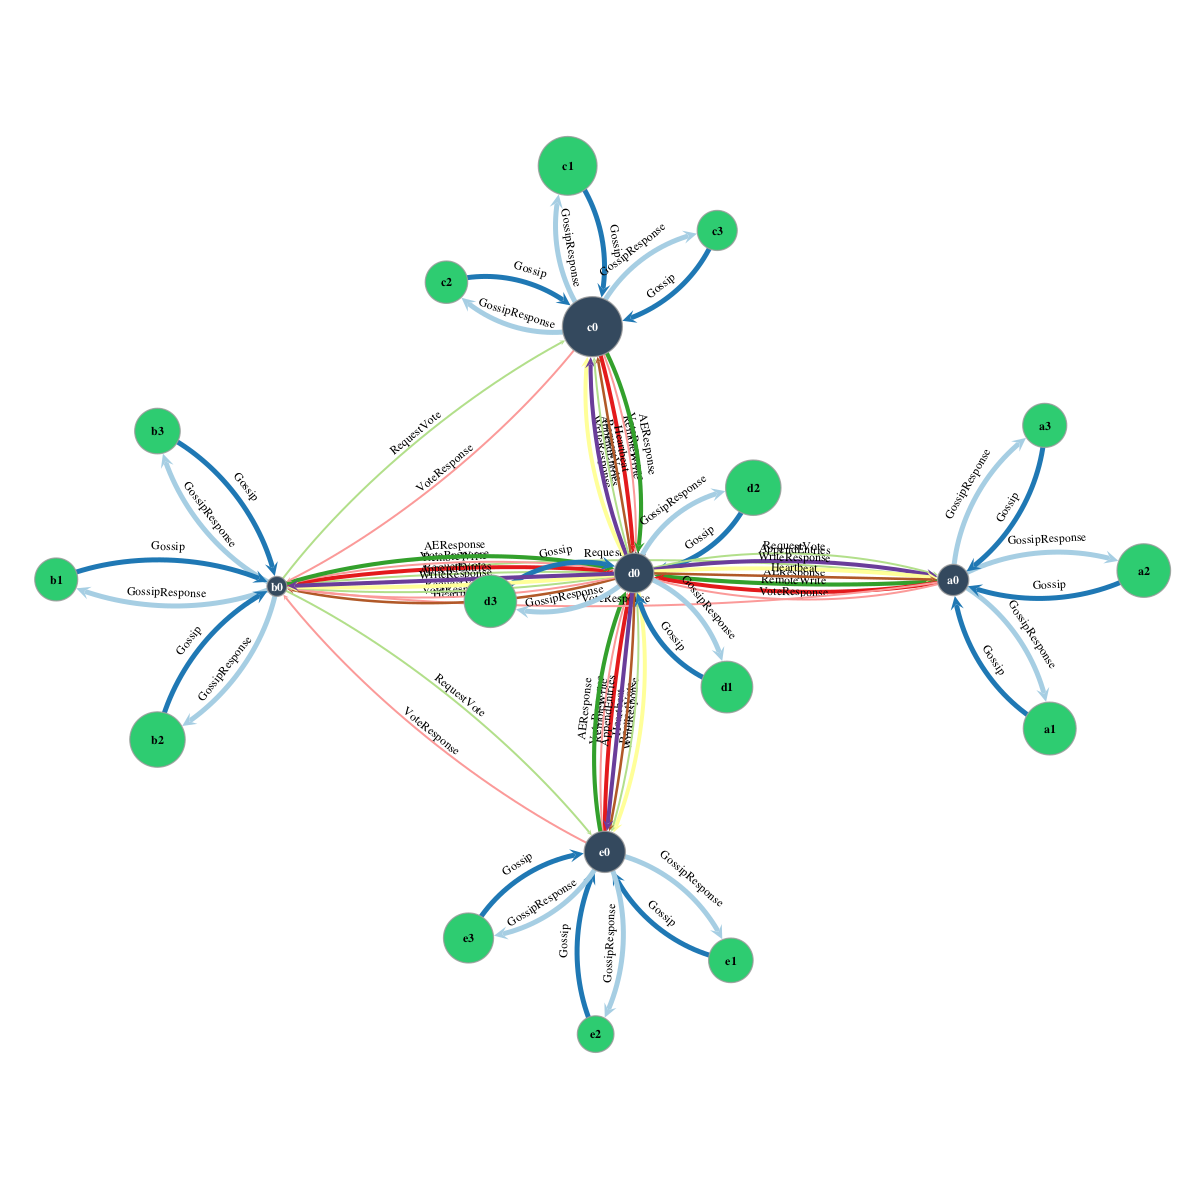
\includegraphics[width=\linewidth]{figures/federated_sync}
    \caption{Communication volume (line thickness) between  heterogeneous replicas in a Federated topology.}
    \label{fig:topology}
\end{figure}

We investigate the effect of variable latency and the network environment on consistency by
constructing a fully connected topology of replicas distributed among several
geographic regions, as shown in Figure \ref{fig:topology}.
Within each region, replicas enjoy stable, low-latency connections with their
neighbors.
The latency is higher and the connections more variable across regions, meaning that
out of order messages are more common across the wide area than in the local area.

\begin{figure*}[t]
    \centering
    \minipage{0.5\textwidth}%
      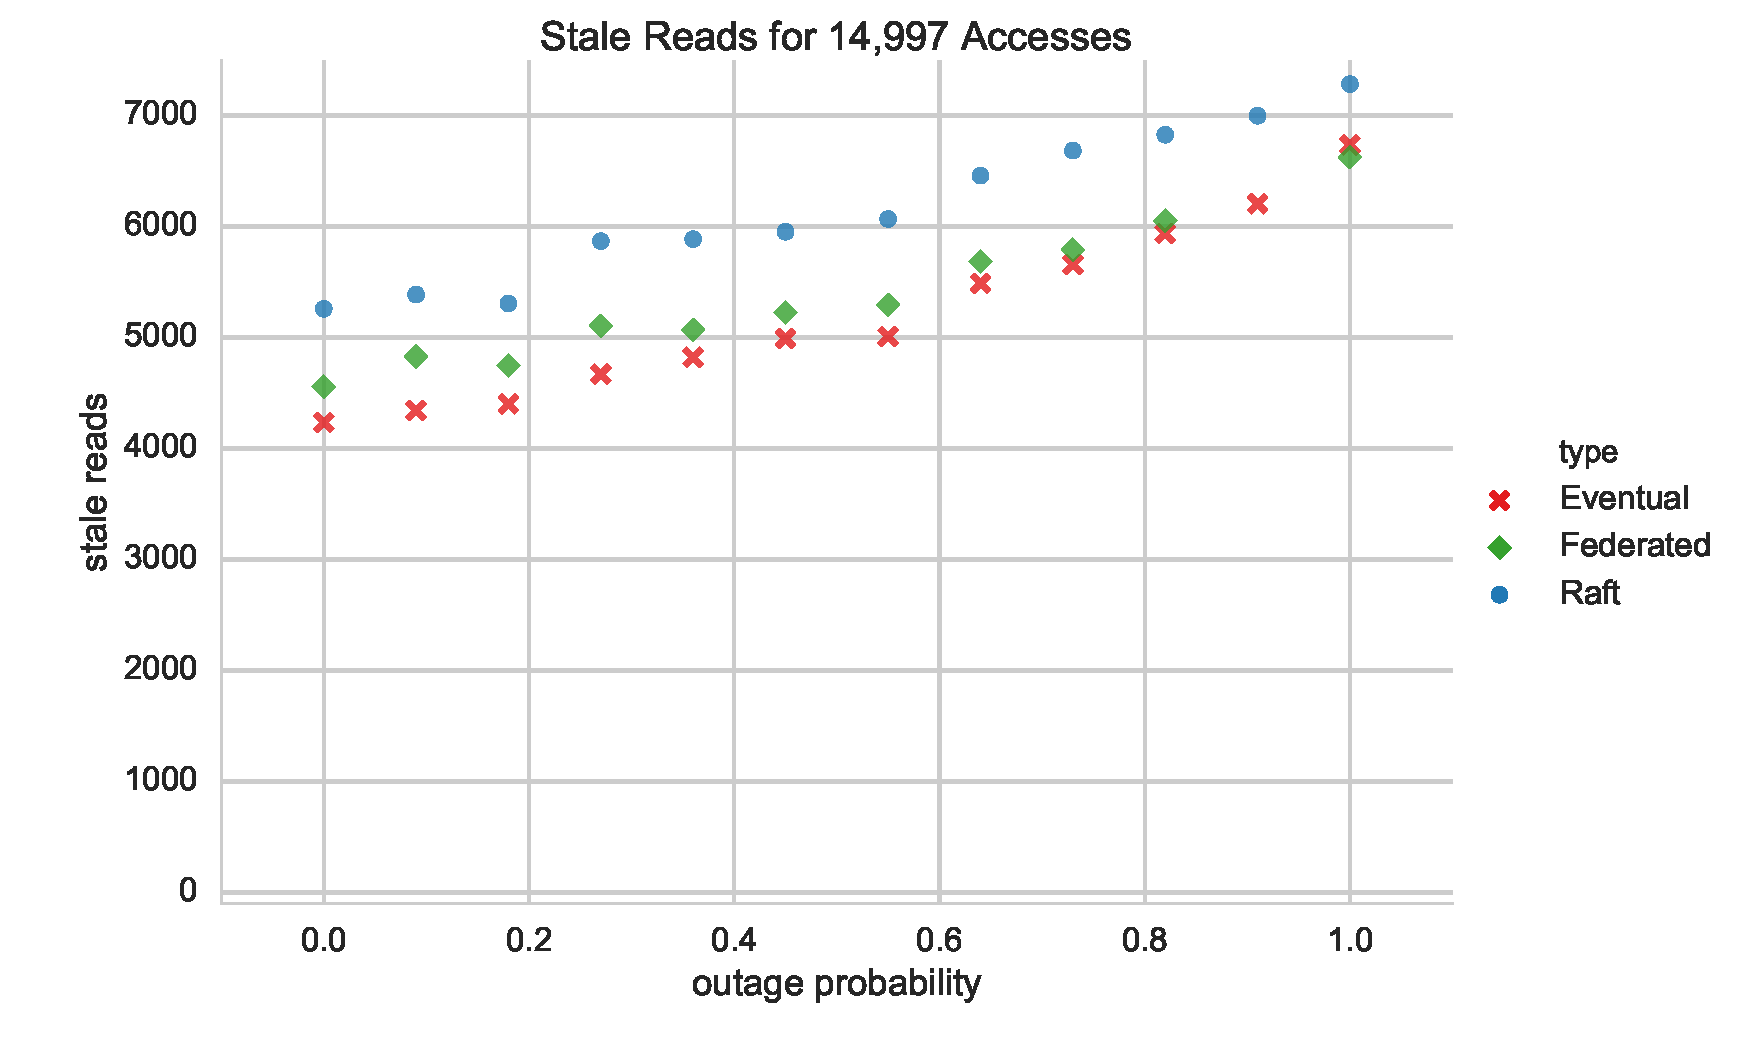
\includegraphics[width=\linewidth]{figures/outages/stale_reads}
      \caption{Stale reads as outages increase.}\label{fig:outages_stale_reads}
    \endminipage
    \minipage{0.5\textwidth}
      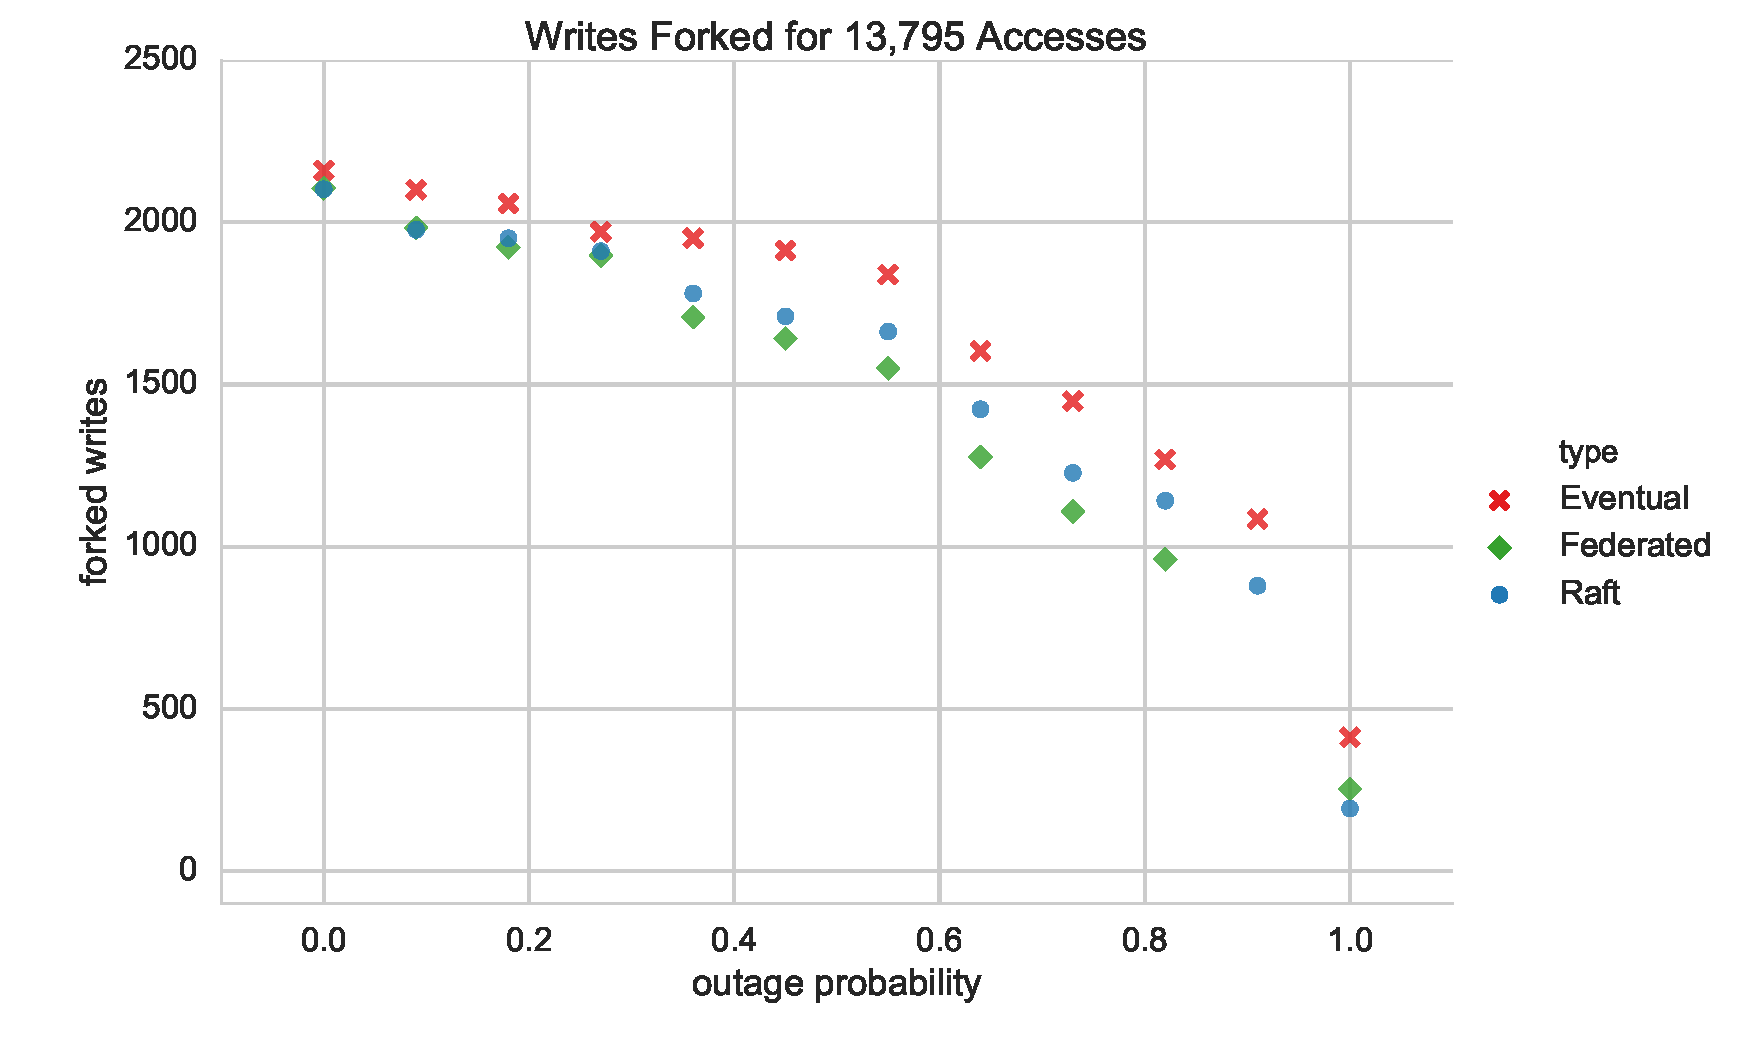
\includegraphics[width=\linewidth]{figures/outages/forked_writes}
      \caption{Forked writes as outages increase.}\label{fig:outages_forked_writes}
    \endminipage\hfill
\end{figure*}

In this type of topology we expect both replica failures, where a single
replica stops responding to messages, and network partitions, where messages
can be exchanged only within geographic regions.
In both cases, accesses may continue within a partitioned replica or subnet
even though they are not immediately replicated in the system.
Partitioned replicas may fall behind the global state, and must be
re-integrated into the network when the network interruption ceases.

% \begin{figure}
%     \centering
%     \minipage{0.5\textwidth}
%       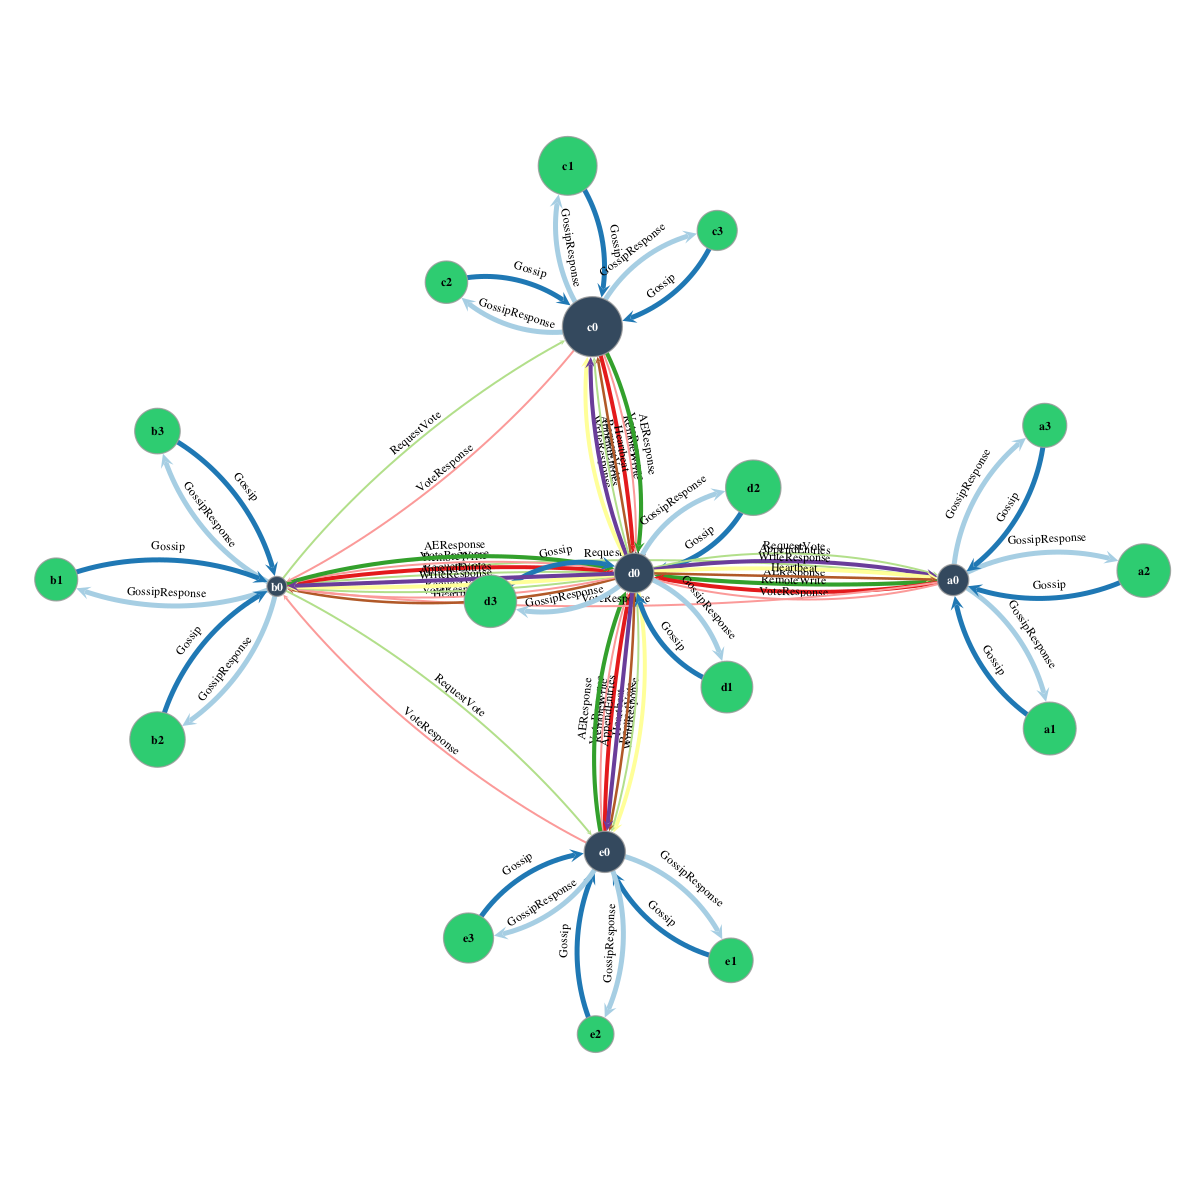
\includegraphics[width=\linewidth]{figures/federated_sync}
%       \caption{Accesses in a Federated topology with primary Raft synchronization.}\label{fig:federated_sync}
%     \endminipage\hfill
%     \minipage{0.5\textwidth}
%       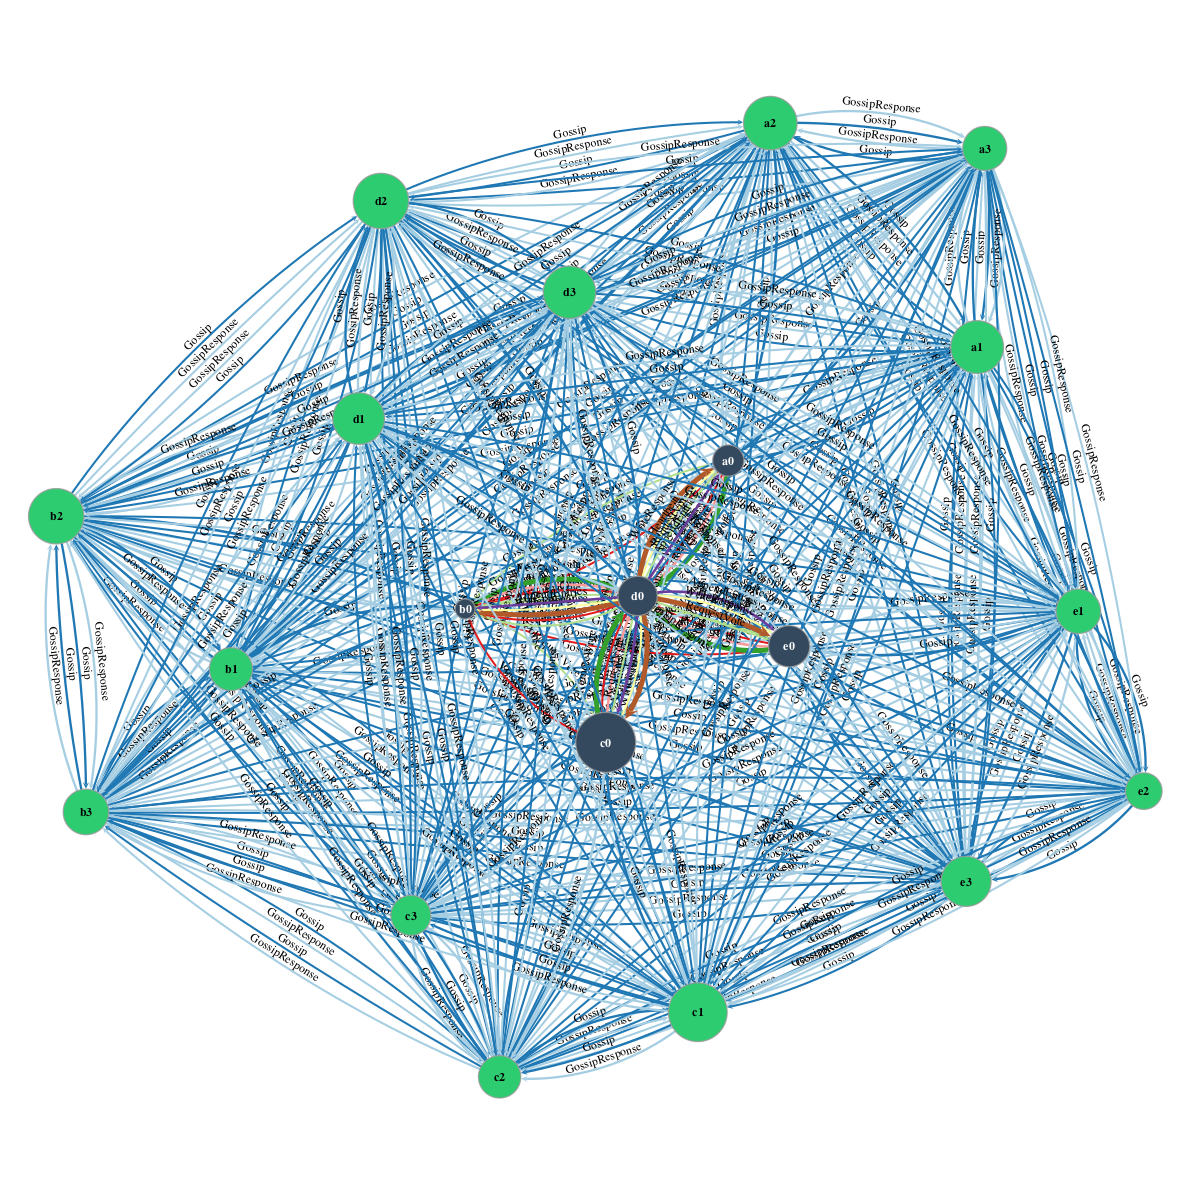
\includegraphics[width=\linewidth]{figures/federated_eventual}
%       \caption{Accesses in a Federated topology with a preference for wide area anti-entropy over synchronization.}\label{fig:federated_eventual}
%     \endminipage\hfill
% \end{figure}

We evaluated the \emph{Federated} model of replication and consistency by creating a
discrete event network simulation that allows us to flexibly configure several parameters.
Simulation input has two parts: a topology that specifies the replicas and
network environment, and a workload of access events to uniquely named objects
(files).
The simulation instantiates each replica as a process that executes read and
write accesses to objects, generates replication messages, and
handles messages from other replicas.
Topologies specify each device as an independent replica by uniquely identifying it
with device-specific configurations.
By far the most important configuration option is a replica's \textit{consistency} (or replication
protocol), which determines the replica's behavior:
\begin{itemize}
    \item \emph{Eventual}: Eventual replicas perform replication via anti-entropy by random
      selection of a neighbor with which to gossip. Eventual  replicas can prioritize
      local vs. wide area replicas by specifying $P_{local}$ -- the likelihood
      of local, versus wide-area, neighbor selection.
    \item \emph{Raft}: Raft replicas implement the Raft consensus protocol, electing a
      leader and forwarding writes to the leader to maintain a sequential
      operation ordering.
      Writes identified as forks of prior committed writes are dropped by
      whichever replica makes the identification.
\end{itemize}

The topology further specifies the \textit{location} of each device, the
\textit{connections} between devices, and the \textit{distribution} of message latency on
a per-connection basis.
Topologies were parameterized with two primary latencies specified as normal distributions ($\lambda_{\mu}$,
$\lambda_{\sigma}$): the \textit{local area} latency, usually with a lower $\lambda_{\mu}$
and $\lambda_{\sigma}$ than the \textit{wide area} latency -- e.g.
the latency between devices in different regions.
In order to compute the tick parameter, $T$, and specify the average latency in the
simulation, latencies are given as worst case, wide-area latencies.
Each topology could also set run- and device-specific configurations, though we
do not use that ability here.

Workloads are specified as access trace files -- time-ordered access events (reads and
writes) between a specific device and a specific object name.
Each trace was constructed via a random workload generator, where a collection of
available devices was specified along with a normal distribution of the delay between
accesses ($A_{\mu}$, $A_{\sigma}$), the number of objects, $o$, in the system, and a
probability of conflict, $P_c$.
To generate the workload, object names were assigned to each replica as follows: in a
round-robin fashion, an object name was selected and assigned to a replica with
probability $P_c$ until each replica was accessing $o$ objects.
If $P_c = 1.0$ then every single replica would be accessing the same batch of objects,
whereas if $P_c = 0.0$ then each replica would access their own unique set of objects.
From there, the $A_{\mu}$, $A_{\sigma}$ was used to generate accesses to objects in
sequence, by selecting an object and reading and writing to it over time until some
probability of switching objects occurred.
In effect, the final workload simulates multiple replicas reading and writing at a
moderate pace for approximately one hour.

In the example topology of Figure~\ref{fig:topology},
the vertex size represents the number of
accesses that occur at a location, and color represents the
replica type.
The edges are colored by RPC type and sized by the
number of messages sent.
Eventual replicas in Federated have a preference for anti-entropy in the local
area cluster, primarily synchronizing across the wide area via Raft replicas.

\begin{figure*}[t]
    \centering
    \minipage{0.5\textwidth}
      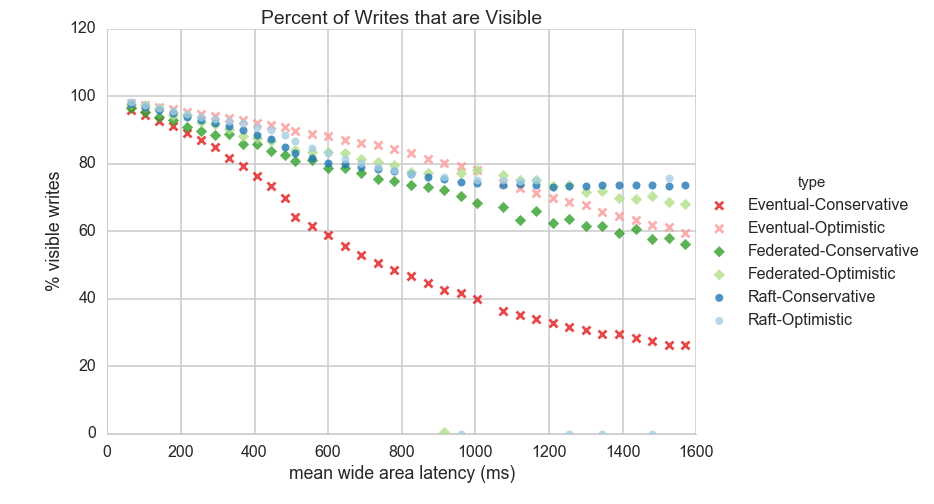
\includegraphics[width=\linewidth]{figures/latency/percent_visible_writes}
      \caption{The percentage of fully visible writes.}\label{fig:visible_writes}
    \endminipage\hfill
    \minipage{0.5\textwidth}
      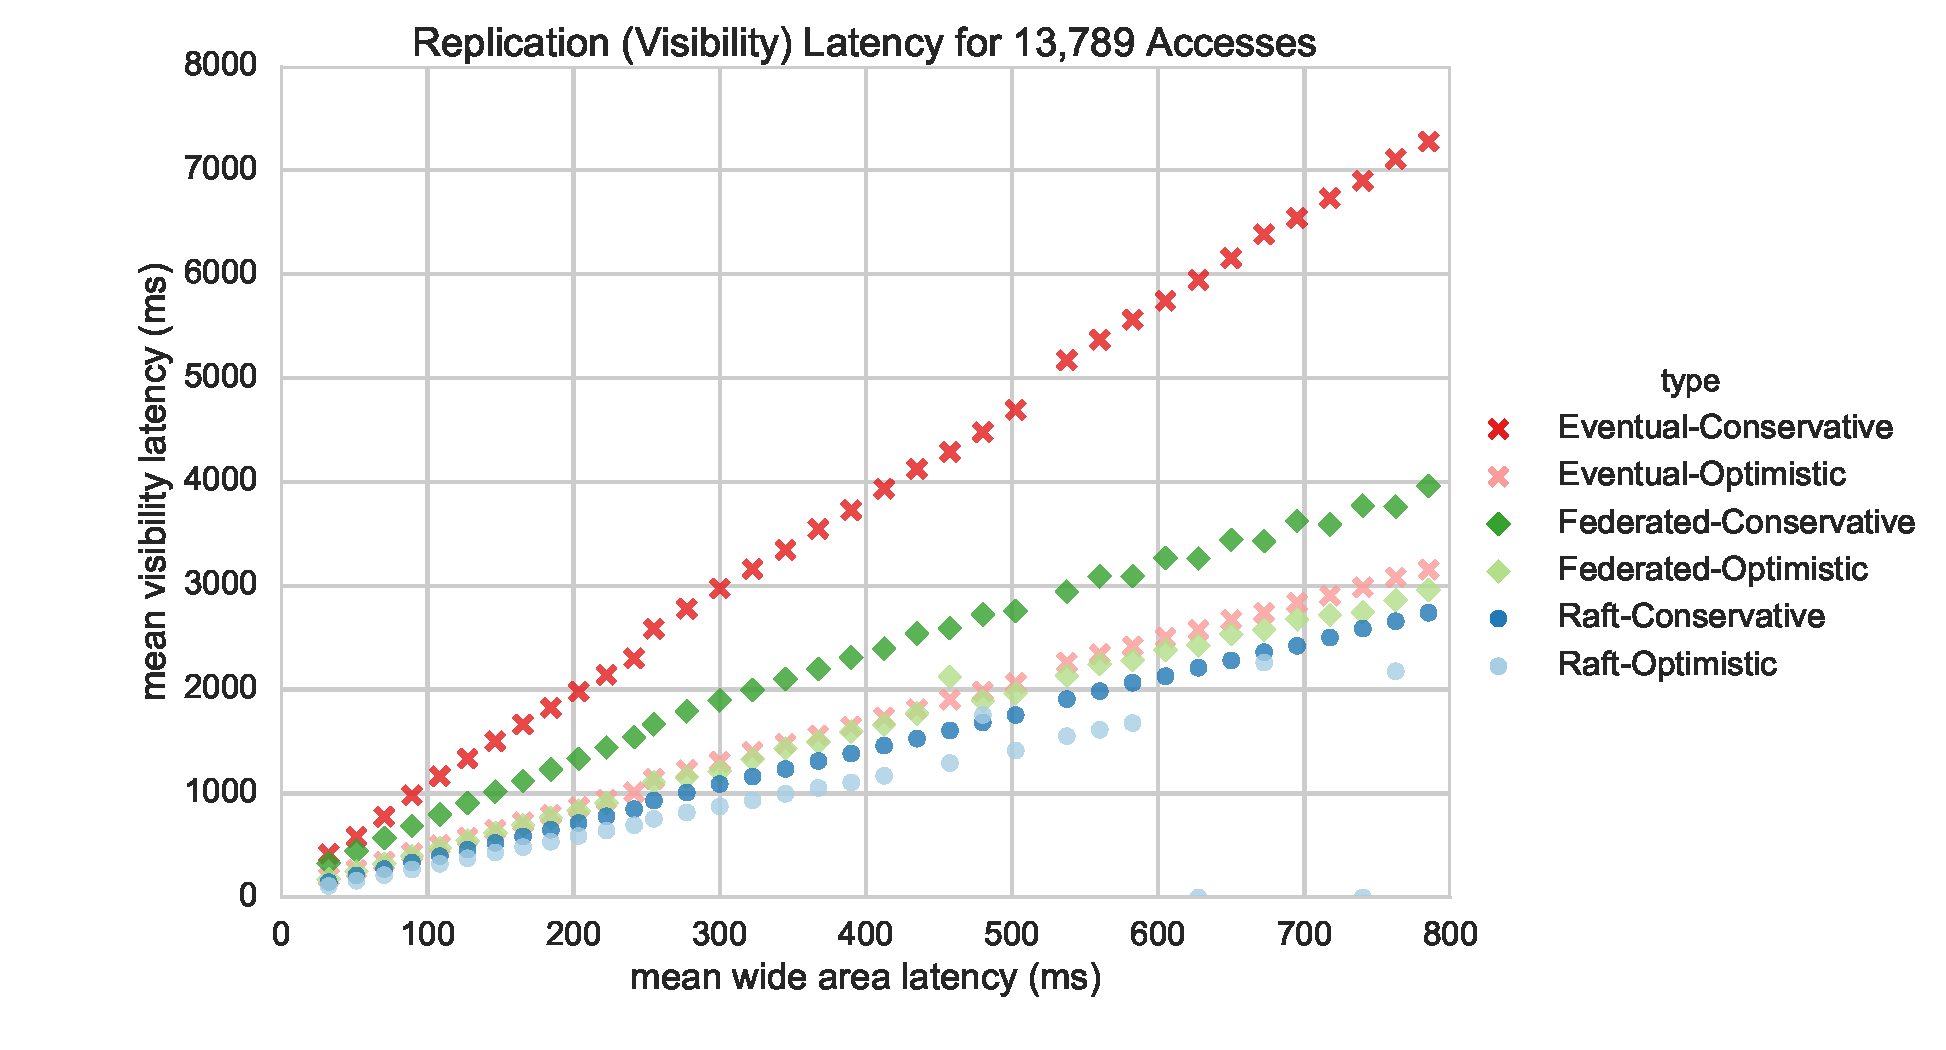
\includegraphics[width=\linewidth]{figures/latency/visibility_latency}
      \caption{The average full visibility latency.}\label{fig:visibility_latency}
    \endminipage\hfill
    \minipage{0.5\textwidth}%
      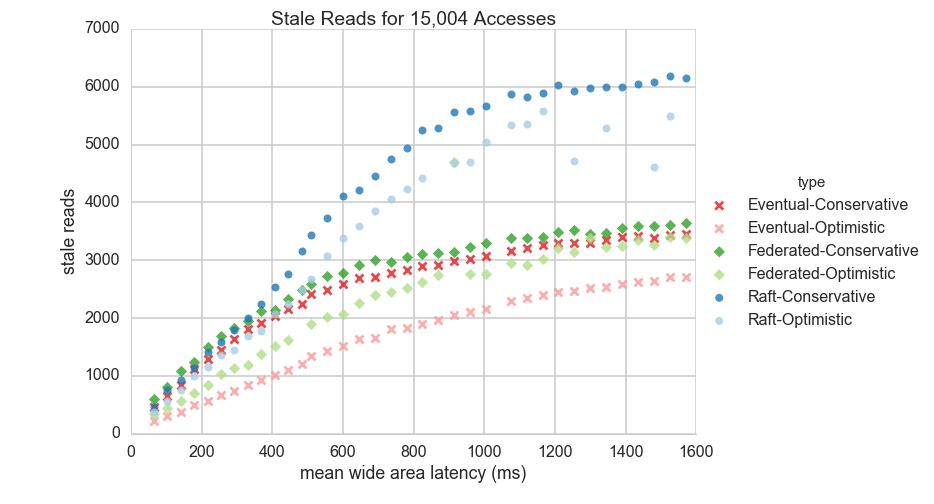
\includegraphics[width=\linewidth]{figures/latency/stale_reads}
      \caption{The percent of reads that are stale in the system.}\label{fig:latency_stale_reads}
    \endminipage
    \minipage{0.5\textwidth}
      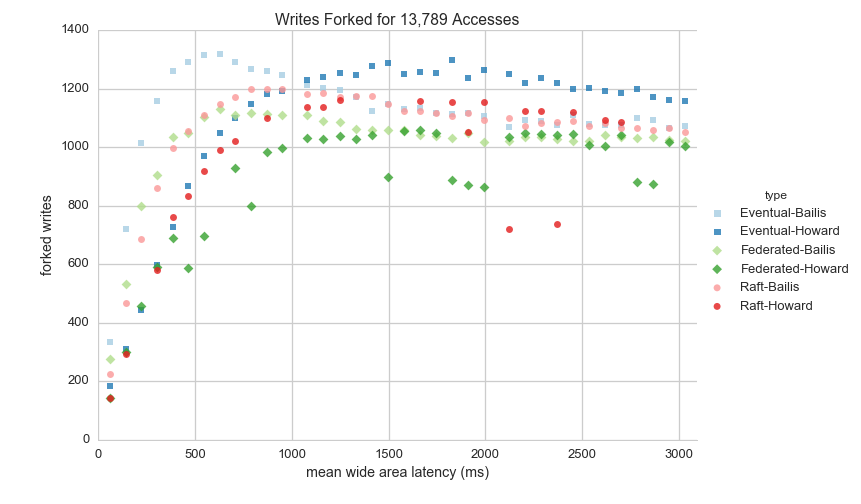
\includegraphics[width=\linewidth]{figures/latency/forked_writes}
      \caption{The total number of conflicts (possible forks).}\label{fig:latency_forked_writes}
    \endminipage\hfill
\end{figure*}

\begin{figure}[t]
    \centering
    \minipage{0.5\textwidth}
      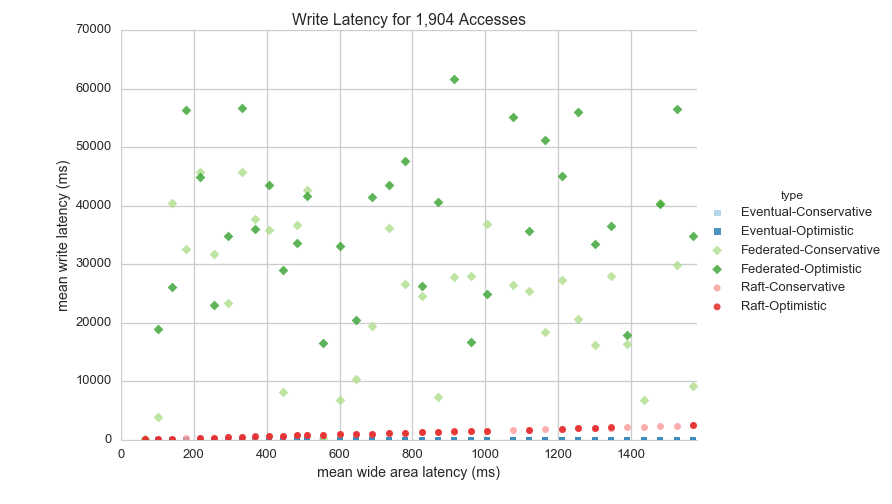
\includegraphics[width=\linewidth]{figures/latency/write_latency}
      \caption{Average local write cost.}\label{fig:write_latency}
    \endminipage\hfill
\end{figure}

\subsection{Experiments and Metrics}

We conducted two primary experiments to test the behavior of a Federated consistency
system against homogeneous Raft and Eventual systems.
The first investigates behavior in the face of increasing failure of wide-area
links, and the
second explores the effect of the network environment in terms of the mean latency,
$\lambda{\mu}$ of the wide area.
Our simulated topology consists of twenty (20) replicas distributed across five (5)
geographic regions.
Eventual replicas prefer other replicas within the same geographic region for
anti-entropy.
Our Federated topology consists of an inner core of Raft replicas distributed one per region,
each co-located with several eventual replicas.
Our experiments were driven by synthetic access traces containing approximately 29,000
accesses (depending on the experiment), approximately two thirds of which are reads.

Our primary metrics are \textit{stale reads} and \textit{forked writes}, which can produce
application-visible effects.
We define forked writes as the number of writes that had more than one child (multiple
writes to the same parent version), whereas reads are stale if they return anything other
than the globally latest version.
We also look at \emph{write visibility}.
Recall that a write is \emph{visible} if and when it is propagated to all replicas.
Any writes that do not become fully visible (stomped on through the eventually consistent
policy of latest writer wins) are ignored.
This metric is closely related to the \textit{percent visible} metric --- the average
number of replicas a write is propagated to.
Finally, we show one graph comparing write latencies.
Read latencies are not meaningful as all read requests are satisfied locally by all of our
protocols, and so have essentially zero latency.

\subsection{Failure Rates}

Figures~\ref{fig:outages_stale_reads} and \ref{fig:outages_forked_writes}
show the effect on stale reads and forked writes
as the probability of wide-area link failures, $P_f \in [0.0,1.0]$, increases
with a step of $0.1$.
A $P_f$ of 0.5 means that all wide-area links are simultaneously down 50\% of
the time,
whereas a $P_f$ of 1.0 means that all wide-area links are permanently down after
a short initial online duration.
Anti-entropy within a single geographic proceeds as usual, though Raft will become unavailable during an outage.

The Eventual system deals with increasingly poor network conditions the best,
as randomized anti-entropy partner selections allow writes to propagate through multiple
paths.
Eventually consistent systems are widely used precisely because of their ability to remain
highly-available despite network failures and
partitions~\cite{bailis_bolt-causal_2013,bailis_probabilistically_2012,bailis_quantifying_2014}.
The Federated system is able to leverage the Eventual subset of its replicas to route
around failures almost as efficiently as the homogeneous Eventual system.

The multiple-paths ability also allows the Federated system to propagate writes quickly,
as shown in Figure~\ref{fig:outages_forked_writes}. In fact, Federated actually outperforms
Eventual, possibly because the Raft quorum is able to quickly disseminate chosen
writes during those periods when wide-area links are available.

The failure mode that we considered took down wide area connections, if
the failure mode was instead random replica failure, the system would respond
differently.
In a quorum size of 5, Raft can handle 2 failures before an extended outage.
Leader failure would cause temporary outages until the election timeout
occurs, but at least one append entries message will be missed.
The central Raft group is therefore the most susceptible part of the system to
random replica failure.
If the Raft replica that fails is a follower, then the eventually consistent
replicas in that area can still make progress without a connection to the
central quorum.
Wide-area anti-entropy will allow updates to be propagated to the entire
network without the central broadcast mechanism.
However, the outage would probably lead to an increase in the number of forks
as reads become increasingly stale with missed pairwise anti-entropy sessions
reducing propagation speed.


\subsection{Latency Variation}


Our second experiment investigates the effect of variable network latency on
consistency protocols, as well as how the selection of the tick parameter
model affects consistency for each system.
% We specified 12 wide area mean latencies in three categories: low ($\lambda{\mu} \in
% [40,500]ms$ with a low $\lambda_{\sigma}=10.0$), medium ($\lambda{\mu} \in [500,1000]ms$
% with a moderate $\lambda_{\sigma}=20.0$), and high ($\lambda{\mu} \in [1000,1500]ms$ with
% a high $\lambda_{\sigma}=30.0$).
In each of these environments we again evaluated three replication models:
\textit{Eventual}, \textit{Raft}, and \textit{Federated}.

Each simulation is parameterized by a $T$ parameter that is a function of the
wide area $\lambda_{\mu}$ and $\lambda_{\sigma}$.
However, the access mean, $A_{\mu}$ was fixed at approximately one access per replica every
3000ms.
In effect, this meant that for approximately half the simulations (with the higher
latencies), it was impossible for a write to become visible on another replica before a
fork.
Even though we fixed the conflict probability as $P_c=0.5$ there was still enough conflict
in the simulation to force each protocol to handle many forks.

% In terms of consistency metrics, the number of inconsistent
% writes\pjk{Again, this is a low-level metric that affects other
% metrics (forks, staleness) that are application/programmer visible.
% We might want to not even mention IWs except to explain strange
% results.}
% is more than halved from Eventual in Federated due to the presence of
% the Raft core (Figure \ref{fig:latency_inconsistent_writes}).
% This is because Federated can take advantage of the topology where
% Raft and Eventual cannot - broadcasting across the wide area to
% minimize the number of pairwise communications in anti-entropy but
% still allowing available responses with the Eventual core.
% Similarly, the number of stale reads as shown in Figure
% \ref{fig:latency_stale_reads} sits between both Raft and Eventual for
% both the optimistic and conservative tick parameters.

Figures~\ref{fig:visible_writes} and \ref{fig:visibility_latency} show that
write propagation is much faster and more effective in Raft than in Eventual,
especially as network conditions deteriorate.
For the mean \emph{replication latency} of writes
(Figure~\ref{fig:visibility_latency}), Federated essentially splits the
difference between Raft and Eventual.
However, Figure~\ref{fig:visible_writes} shows that Federated fully replicates
many more writes than Eventual, closely tracking the number of writes fully
replicated by Raft.

The strong inner core of Raft replicas is the key to the Federated protocol
tracking Raft's performance.
Eventual replicas are biased in favor of performing anti-entropy with local
replicas, allowing most anti-entropy sessions to perform quickly and without
delay.
By contrast, the Raft replicas in our Federated topology are intentionally
spread across geographic regions.
A new write originating at an Eventual replica is quickly spread to the local
Raft replica, and is then broadcast to the rest of the regions via the Raft
\texttt{AppendEntries} message.
Disseminating writes quickly minimizes the possibility of another, later
Eventual write starting up concurrently.
Additionally, the Forte number prevents new forked writes from stomping on a
conflicting write disseminated via Raft replicas.

Figures~\ref{fig:latency_stale_reads} and \ref{fig:latency_forked_writes} show
the average number of stale reads and forked writes across different mean
latencies.
All three protocols perform similarly at smaller latencies, but Eventual and
Federated deal with high latencies much more effectively than Raft, at least
for this size of system.

Higher latencies affect Raft in at least two ways.
First, higher latency variability causes more out of order messages.
Second, we parameterize system timeouts by $T$ which, in turn, is based on
mean latencies.
The result is that Raft's \texttt{AppendEntries} delay is longer for
simulations with higher mean latencies, resulting in more conflicts.
The same is true for anti-entropy delays, but the speed of Raft decisions is
determined by the slowest quorum member, which can be quite slow when message
variability is large.
By contrast, a slow anti-entropy participant only affects direct anti-entropy
partners.

Though not shown here, we also investigated the effect of changing the number
of replicas in the system.
As system size increases, more time is required to fully replicate writes,
increasing the likelihood of both stale reads and forks.
Equation~\ref{eq:propagation} shows that bilateral anti-entropy propagates writes
to $N$ nodes exponentially.
Given the relationship of the \texttt{anti-entropy delay} and \texttt{heartbeat interval}
expressed by $T$, Raft broadcasts overtake anti-entropy between 9 (2 anti-entropy
sessions) and 27 replicas (3 anti-entropy sessions).
% In simulations of 20 replicas, these figures show not only the consequences of
% replication latency, but also the impact of consistency policies on both staleness and
% forks.

% Ben is hinting at an expectation that was more fig 8 (forks) than 7 (stale
% reads). At higher system sizes we'd expect them to look more similar.

Figure~\ref{fig:write_latency} shows the mean synchronous cost of write operations to
ongoing computations.
All Raft writes must be forwarded to the leader in order to be serialized and are
completed after a round trip communication.
Eventual writes are local and are completed immediately, even before being replicated,
and therefore have zero write cost.
Most Federated replicas are Eventual and therefore Federated's average write cost tracks
Eventual's relatively closely.

\section{Related Work}
\label{sec:related}

One of the earliest attempts to hybridize weak and strong consistency was a
model for parallel programming on shared memory systems by Agrawal et al
\cite{agrawal_mixed_1994}.
This model allowed programmers to relax strong consistency in certain contexts
with causal memory or pipelined random access in order to improve parallel
performance of applications.
Per-operation consistency was extended to distributed storage by the RedBlue
consistency model of Li et al \cite{li_making_2012}.
Here, replication operations are broken down into small, commutative
sub-operations that are classified as red (must be executed in the same order
on all replicas) or blue (execution order can vary from site to site), so long
as the dependencies of each sub-operation are maintained.
The consistency model is therefore global, specified by the red/blue ordering
and can be adapted by redefining the ratio of red to blue operations, e.g.
all blue operations is an eventually consistent system and all red is
sequential.

The next level above per-operation consistency hybridization is called
\textit{consistency rationing} wherein individual objects or groups of objects
have different consistency levels applied to them to create a global quality
of service guarantee.
Kraska et al.
\cite{kraska_consistency_2009} initially proposed consistency rationing be on
a per-transaction basis by classifying objects in three tiers: eventual,
adaptable, and linearizable.
Objects in the first and last groups were automatically assigned transaction
semantics that maintained that level of consistency; however objects assigned
the adaptable categorization had their consistency policies switched at
runtime based on a cost function that either minimized time or write costs
depending on user preference.
This allowed consistency in the adaptable tier to be flexible and responsive
to usage.

Chihoub et al.
extended the idea of consistency rationing and proposed limiting the number of
stale reads or the automatic minimization of some consistency cost metric by
using reporting and consistency levels already established in existing
databases \cite{chihoub_harmony:_2012,chihoub_consistency_2013}.
Here multiple consistency levels are being utilized, but only one consistency
model is employed at any given time for all objects, relaxing or strengthening
depending on observed costs.
By utilizing all possible consistency semantics in the database, this model
allows a greater spectrum of consistency guarantees that adapt at runtime.

Al-Ekram and Holt \cite{al-ekram_multi-consistency_2010} propose a middleware
based scheme to allow multiple consistency models in a single distributed
storage system.
They identify a similar range of consistency models, but use a middleware
layer to forward client requests to an available replica that maintains
consistency at the lowest required criteria by the client.
However, although their work can be extended to deploying several consistency
models in one system, they still expect a homogeneous consistency model that
can be swapped out on demand as client requirements change.
Additionally their view of the ordering of updates of a system is from one
versioned state to another and they apply their consistency reasoning to the
divergence of a local replica's state version and the global version.
Similar to SUNDR, proposed by Li et al.
\cite{li_secure_2004}, an inconsistency is a fork in the global ordering of
reads and writes (a ``history fork'').
Our consistency model instead considers object forks, a more granular level
that allows concurrent access to different objects without conflict while
still ensuring that no history forks can happen.

\balance

Hybridization and adaptation build upon previous work that strictly
categorizes different consistency schemes.
An alternative approach is to view consistency along a continuous scale with
several axes that can be tuned precisely.
Yu and Vahdat \cite{yu_design_2002} propose the \textit{conit}, a consistency
unit described as a three dimensional vector that describes tolerable
deviations from linearizability along staleness, order error, and numeric
ordering.
Similarly, Afek et al.
\cite{afek_quasi-linearizability:_2010} present quasi-linearizable histories
which specify a bound on the relative movement of ordered items in a log which
make it legally sequential.

A strong central core to provide support to the entire system has been
suggested both in Oceanstore \cite{kubiatowicz_oceanstore:_2000} and primary
copy schemes \cite{gray_dangers_1996}.
We take this idea further in our experiments by Federating a strong central
core composed of Replicas that perform consensus via the Raft consensus
protocol and combine it with highly available eventually consistent systems.
In this way Federated consistency gains the flexibility and availability of
the Eventual replicas (leader re-election and no requirement for remote writes
mean that the replica can continue even if it is completely partitioned from
the rest of the network) while still getting guarantees from Raft, which
minimizes ``fork flipping'' -- the behavior of writing to one branch then
another, truly pernicious inconsistent behavior that cannot be prevented in an
eventually consistent system.

System designers can take advantage of heterogeneous replicas by implementing
stronger consistency on more reliable machines that are able to handle more
messages.
Mobile replicas that are prone to network loss, out of order or missed
messages, or other variable behavior can adapt their policy depending on the
environment they're in.
Our model also allows for \textit{adaptive} behavior, in that the replicas can
monitor the environment for change and as the mean latency decreases, adapt
their $T$ parameter accordingly.
This is a no cost operation for Eventual replicas (who can also optimize
pairwise gossip by implementing non-discrete random selection using Bandits or
other optimization techniques), and only requires joint consensus on the part
of the consensus group.

\vspace{.5em}
\section{Discussion \& Conclusion}
\label{sec:conclusion}

This paper has presented a model for Federated consistency, which allows individual
replicas to expose local policies to users, while still allowing for global guarantees.
We evaluate Federated consistency in the context of a geographically dispersed wide-area
file system.
Our results show that a key to the global guarantees is in using a core
strongly-consistent group to serialize and broadcast system writes.
By designing a Federated system where only the interactions between replicas of varying
consistency types are defined, systems can scale beyond the handful of devices usually
described to dozens or hundreds of replicas in variable-latency, partition-prone
geographic networks.
Replicas can monitor their local environment and adapt as necessary to meet timeliness and
correctness constraints required by the local user.

We were only able to investigate a limited number of system configurations,
and this paper has space for even fewer.
However, the space of possible system configurations is vast.
We do not claim that the configurations described in this paper are in any way
optimal. Rather, we claim that the extremely promising results described in
Section~\ref{sec:results} show that the general approach is promising.
Our simulation environment is extremely flexible, and we intend to continue
evaluating possible system configurations as we move towards building a
wide-area file system in this environment.

One particularly intriguing option we are evaluating is scaling Federated system size
upwards.
The central Raft quorum must also scale, but increased quorum sizes often degrade
performance as the leader becomes a bottleneck.
Additionally, the Raft quorum in our topology does not benefit from localization, as do
the eventually consistent replicas.
% It is possible that placing all of the Raft replicas in a single location,
% giving Raft RPC messages the benefit of the local area connections and
% penalizing the synchronization of wide area Eventual replicas, would have
% increased the overall performance of the system.
% Because of the centrality of the Raft quorum in providing stronger consistency
% guarantees in a Federated environment, we propose future work into optimizing
% coordination for user-centric dynamic networks.
We are therefore investigating approaches to \emph{hierarchical consensus}, which will
allow Raft to maintain smaller quorum sizes and localize decision making while scaling to
larger systems.

% \section*{Acknowledgments}
%
% Thank you Bluejacket, for tirelessly running simulations as soon as we spun you up.

\newpage
\bibliographystyle{plain}
\bibliography{references}


\end{document}
